%%%%%%%%%%%%%%%%%%%%%%%%%%%%%%%%%%%%%%%%%%%%%%%%%%%%%%%%%%%%
%%%%%            CAMPFIRE Readme file                  %%%%%
%%%%%%%%%%%%%%%%%%%%%%%%%%%%%%%%%%%%%%%%%%%%%%%%%%%%%%%%%%%%
%%%%%  History:                                        %%%%%
%%%%%   Original text: Chris Goodyer, May 2012         %%%%%
%%%%%   Latest version - Chris Goodyer, September 2012 %%%%%
%%%%%%%%%%%%%%%%%%%%%%%%%%%%%%%%%%%%%%%%%%%%%%%%%%%%%%%%%%%%
% ------------------------------------------------------------------------------
% The format is based on: 
%         LaTeX Template: Titlepage
%         This is a title page template which be used for both articles and reports.
%
%         Copyright: http://www.howtotex.com/
%         Date: April 2011
% ------------------------------------------------------------------------------

% -------------------------------------------------------------------------------
% Preamble
% -------------------------------------------------------------------------------
\documentclass[paper=a4, fontsize=11pt,twoside,bibtotoc]{scrartcl}		% KOMA article
\usepackage[a4paper,pdftex]{geometry}					% A4paper margins
\setlength{\oddsidemargin}{5mm}						% Remove 'twosided' indentation
\setlength{\evensidemargin}{5mm}

\usepackage[english]{babel}
%\usepackage[protrusion=true,expansion=true]{microtype}	
\usepackage{amsmath,amsfonts,amsthm,amssymb}
\usepackage{graphicx}

%% Custom sectioning (sectsty package)
\usepackage{sectsty}                                    % Custom sectioning (see below)
\allsectionsfont{\centering \normalfont\scshape}        % Change font of al section commands

\usepackage{framed}
\usepackage{bold-extra}
\usepackage{longtable}

% ------------------------------------------------------------------------------
% Definitions (do not change this)
% ------------------------------------------------------------------------------
\newcommand{\HRule}[1]{\rule{\linewidth}{#1}} 	% Horizontal rule

\makeatletter							% Title
\def\printtitle{%						
    {\centering \@title\par}}
\makeatother									

\makeatletter							% Author
\def\printauthor{%					
    {\centering \large \@author}}				
\makeatother							

% ------------------------------------------------------------------------------
% Metadata (Change this)
% ------------------------------------------------------------------------------
\title{	\normalsize \textsc{Campfire : Users and Developers Guide} 	% Subtitle of the document
		 	\\[1.0cm]									% 2cm spacing
			\HRule{2pt} \\										% Upper rule
			\Huge \textbf{\uppercase{CAMPFIRE}}\\	% Title
			\Large \textbf{\uppercase{Campfire: Adaptive, Multilevel, Parallel\\ Fully Implicit Research Engine }}	% Title
			\HRule{2pt} \\ [0.5cm]								% Lower rule + 0.5cm spacing
			\normalsize %\today									% Todays date
		}

\author{
		Christopher Goodyer\\	
		School of Computing\\	
		University of Leeds\\
        \texttt{C.E.Goodyer@leeds.ac.uk} \\
}

%\usepackage{scrpage}
\usepackage[automark]{scrpage2} % This should be set AFTER setting up the page geometry
\pagestyle{scrheadings}
% \ohead{\pagemark} 
 \cehead{CAMPFIRE} 
 \cohead{Users and Developers Guide} 
 \ofoot[]{} 
 \cofoot[]{\pagemark} 
 \cefoot[]{\pagemark} 
%\makeatletter
%  \markboth{Left}{Right}
%\makeatother

\lehead{\rightmark}

\newcommand{\CiteParamesh}{\cite{paramesh1,paramesh2, paramesh3}}

% ------------------------------------------------------------------------------
% Macros
% ------------------------------------------------------------------------------
%\newenvironment{codebox}{\begin{center}\begin{framed}[0.75\linewidth]\tt}{\end{framed}\end{center}}
\newenvironment{codebox}{\begin{center}\begin{MakeFramed}{\hsize0.99\linewidth\advance\hsize-\width\FrameRestore}\tt}{\end{MakeFramed}\end{center}}
\newenvironment{filebox}{\begin{center}\begin{MakeFramed}{\hsize0.99\linewidth\advance\hsize-\width\FrameRestore}\tt\begin{tabular}{l}}{\end{tabular}\end{MakeFramed}\end{center}}
\newcommand{\prompt}[1]{\textsl{\%} \textbf{#1}}
\newcommand{\exclude}[1]{}



\begin{document}

% ------------------------------------------------------------------------------
% Maketitle
% ------------------------------------------------------------------------------
\thispagestyle{empty}				% Remove page numbering on this page

\printtitle									% Print the title data as defined above
  	\vfill
\printauthor								% Print the author data as defined above
  	\vfill

\newpage

\tableofcontents

\clearpage
% ------------------------------------------------------------------------------
% Begin document
% ------------------------------------------------------------------------------

\section{Introduction}

Campfire is a tool to facilitate coupling non-linear multigrid, parallel execution on a properly load balanced adaptively refined grid, using the open source 
library PARAMESH~\CiteParamesh.  
The intention is to provide a user-friendly interface layer where only the application-specific routines are exposed to the user by default.
Obviously the source to the library is also provided and it is envisaged that there may be future scenarios where applications may need to extend the functionality 
of the main algorithm.

PARAMESH, as used here, is an adaptive mesh refinement code which works on individual square/cubic blocks of data.  These data blocks therefore can be spread 
across processors allowing parallelism.  This is accomplished using MPI.  Since each block is independent in memory from its neighbours they all have a layer of 
\textsl{guard cells} around the outside which can be filled with the appropriate neighbouring values.  PARAMESH includes its adaptivity through quad-tree/oct-tree
uniform refinement of blocks.

By default PARAMESH includes a linear multigrid solver in its code-base, although this not used by default.
Campfire extends this idea to be an FAS multigrid in order to solve non-linear equations.
The mesh refinement functionality in PARAMESH allows the multigrid implementation to therefore be an adaptive mesh multigrid, sometimes coined MLAT.

The use of multigrid in Campfire inherently needs a smoother to be applied at each level.  A Jacobi pointwise finite difference smoother is used, with an 
approximate solve performed on the coarsest grid level.

This document is structured as follows.  In Section~\ref{SEC_History} more details of the genesis of this software are given, along with information on how it 
operates.  The changes from the default PARAMESH behaviour are also summarised.

Instructions on how to obtain, and compile the code is given in~\ref{SEC_Compiling} with the additional information for running cases given in 
Section~\ref{SEC_Running}. 

Information for developers follows.  In Section~\ref{SEC_Existing} guidelines on extending existing models is given, and Section~\ref{SEC_New} explains how to 
write a new application.

Contained in Campfire are a collection  of tools intended to aid visualization of outputs.  These are described in Section~\ref{SEC_Viz}.  There are also a 
growing number of documents included with the software in the \texttt{DOCS} directory and the suggestions for how to add what to these are given 
in Section~\ref{SEC_Documentation}.

Finally the document concludes with a full description of the API (Section~\ref{SEC_API}), known bugs and features needed to be added (Section~\ref{SEC_Bugs}).


%%%%%%%%%%%%%%%%%%%%%%%%%%%%%%%%%%%%%%%%%%%%%%%%%%%%%%%%%%%%%%%%%%%%%%%%%%%%%%%%%%%%%%%%%%%%%%%%%%%%%%%%%%%%%%%%%%%%%%%%%%%%%%%%%%%%%%%%%%%%%%%%%%%%%%%%%%%%%%%%%%%
\section{History and Implementation}	
								\label{SEC_History}

Following the development of a 2-d fully implicit adaptive multigrid code for phase field problems~\cite{janref1,janref2,janref3}, now released as open source 
software from~\cite{jancode} attention turned to the more interesting, but considerably more computationally challenging 3-d problems.  The need for multigrid, 
adaptive meshing and implicit timestepping had been clearly demonstrated, but in order to get to mesh resolutions that were sufficiently fine to be realistic, but 
sufficiently large domains to be useful then a move to a parallel implementation was imperative.  As such, PARAMESH was chosen as a suitable software library 
providing a necessary framework in which to build these applications.

The PARAMESH software used in this work was developed at the NASA Goddard Space Flight Center and Drexel University under NASA's HPCC and ESTO/CT projects and 
under grant NNG04GP79G from the NASA/AISR project.

The original development of what is today the Campfire software was done by Jan Rosam and James Green.  This resulted in a software basis that forms much of the 
core code present today in Campfire.  In particular many of the components of both the MG-SRC and PF-SRC directories come from their work.  Chris Goodyer took 
their software, corrected many issues and has repackaged it as given here.  The major extensions are as described in the following paragraphs.

This idea of adaptive meshes for multigrid is one of the most important areas where the original PARAMESH library has had to be modified.  
For efficient parallelism there needs to be equal work distribution per processors on every grid.  Unfortunately the default PARAMESH implementation has a load 
balancing of all the blocks in the simulation, irregardless of which grid is being worked on.  A new algorithm was devised, throwing away the Morton ordering that 
PARAMESH has at its heart, and ordering the blocks per processor based on which grid they are on.  In order to load balance the first and last blocks on that 
processor are shuffled left or right if a processor has too many blocks.

Whilst apative meshing is included in the default mesh it requires that the domain remains fixed throughout the computation.  For most simulations this is entirely 
sensible.  However for the phase field applictions that this software suite was designed for this is not quite so useful.  The simulation is about growing a 
dendrite from a small seed.  Fixing the domain means that the total mesh requirements of the final solution need to be known before starting the simulation.  In 
order to combat this requirement a mesh growing strategy has been introduced.  The basic idea is that as the solution grows towards a far-field boundary condition 
extra blocks are added on the coarsest level to allow the solution to keep growing.  Advantages of this approach are that the simulation can be started on a very 
small domain and be allowed to adapt as necessary, and that this adaptation need no longer be constrained to square domains.  The introduction of non-convex 
corners meant that further changes were necessary in the PARAMESH library, as did the loading of checkpoint files with different domain sizes than the initial 
domain specified in the setup procedures.

The simulations undertaken using Campfire are time-dependent.  By default they use BDF2, so use two previous timesteps in addition to the new step being 
calculated.  Adaptive timestepping is included by default, either based on convergence of individual steps, or on a local error estimation technique.



%%%%%%%%%%%%%%%%%%%%%%%%%%%%%%%%%%%%%%%%%%%%%%%%%%%%%%%%%%%%%%%%%%%%%%%%%%%%%%%%%%%%%%%%%%%%%%%%%%%%%%%%%%%%%%%%%%%%%%%%%%%%%%%%%%%%%%%%%%%%%%%%%%%%%%%%%%%%%%%%%%%

\section{Installation and Compilation}
								\label{SEC_Compiling}

\exclude{        Make Paramesh with "make -f Makefile.Intel".
        You may need to tweak some directories in various Makefile places 
        for these.

HDF5

        http://www.hdfgroup.org/ftp/HDF5/prev-releases/hdf5-1.6.10/src/

        Configure with

                ./configure --enable-parallel
--prefix=/usr/not-backed-up/PHASEFIELD/hdf5-1.6.10 CC=mpicc F90=mpif90

        (with appropriately named prefix address)

Paramesh documentation:

        http://www.physics.drexel.edu/~olson/paramesh-doc/Users_manual/amr.html
}


For the sake of simplicity here I am assuming that all code is going to be installed in \texttt{/usr/not-backed-up/} on a linux machine.  You should obviously 
pick somewhere appropriate, and never leave important work on an unbacked up filesystem.

The first thing that needs to happen is obtaining the appropriate (latest) versions of the software.  This comes in three parts: Paramesh, Campfire and (an old) 
HF5 library.

The latest versions of both Paramesh and Campfire that should be used together live on an SVN repository at the University of Leeds.  If you havn't already been 
granted access to this contact \texttt{support@comp.leeds.ac.uk}, IT Support in the Faculty of Engineering, explaining what 
you need and why.  They will also be able to organise access to the university's \textsl{Trac} server,  through which we do the issue management.

In order get these latest versions then the appropriate commands are:

\begin{codebox}
        \prompt{svn checkout https://repo.engineering.leeds.ac.uk/svn/paramesh}

        \prompt{svn checkout https://repo.engineering.leeds.ac.uk/svn/Campfire}
\end{codebox}

\noindent which should be run from your chosen directory.  Before proceeding further it is necessary to take a detour into another library.

\subsection{HDF5}

For checkpointing files Paramesh uses the HDF5 library.  However, it is an old version using commands 
that are now no longer included in the latest versions.  As such you should download a version prefixed 1-6.  I suggest getting 1-6.10 using

\begin{codebox}
	\prompt{wget http://www.hdfgroup.org/ftp/HDF5/prev-releases/ hdf5-1.6.10/src/hdf5-1.6.10.tar.gz}
\end{codebox}

In order to compile this it is first necessary to unpack this gzipped tarball, then proceed to configure the Makefile, compile and install.  

\begin{codebox}
	\prompt{tar xvzf hdf5-1.6.10.tar.gz}

	\prompt{cd hdf5-1.6.10}

        \prompt{make distclean}

        \prompt{./configure --enable-parallel --prefix=/usr/not-backed-up/hdf5-1.6.10 CC=mpicc F90=mpif90}

        \prompt{make}

        \prompt{make install}
\end{codebox}

The addition of \texttt{-fPIC} flag into the CFLAGS list in the Makefile may be necessary for compilation when using the \texttt{libtool}-compiled libraries that 
follow.

\subsection{Environment variables}

In order to help keep the Makefiles used as generic as possible we have set them up to use two environment variables to denote the location of the Paramesh and 
Campfire directories on the installed system.  Therefore \texttt{tsch} users should set the following in their \texttt{~/.cshrc} file:

\begin{codebox}
       	setenv HDF5\_DIR /usr/not-backed-up/hdf5-1.6.10

        setenv PARAMESH\_DIR /usr/not-backed-up/paramesh
\end{codebox}

\noindent and \texttt{bash} users should set	the following in their \texttt{~/.bashrc} file:
\begin{codebox}
        export HDF5\_DIR=/usr/not-backed-up/hdf5-1.6.10

        export PARAMESH\_DIR=/usr/not-backed-up/paramesh
\end{codebox}

\noindent New login shells (terminal windows) should be started before doing the next installs.


\subsection{Paramesh}

In order to check your environment variable is set correctly we can do:

\begin{codebox}
	\prompt{cd \$PARAMESH\_DIR}

	\prompt{ln -s Makefile.Intel Makefile}

	\prompt{make -j 16}
\end{codebox}

Hopefully this should all compile without issues.  If you are using a system with shared libraries then the contents of \texttt{\$PARAMESH\_DIR/lib} should look 
like:
\begin{codebox}
	\prompt{ls \$PARAMESH\_DIR/lib}

	libmodules.a   libmpi\_paramesh.a   libparamesh.a
	libmodules.so  libmpi\_paramesh.so  libparamesh.so
\end{codebox}
whereas on systems without (such as HECToR) none of the \texttt{lib*.so} files will have been created.

Note that the \texttt{ln -s Makefile.Intel Makefile} line above is important.  Currently the link is not included by default allowing users to choose their own 
compiler without polluting the SVN repository for others.  A creating of a \texttt{Makefile} is needed, however, for the code to compile without issues.

\subsection{Campfire}

Compiling the Campfire library and all the applications that come with it is achieved by simply typing:

\begin{codebox}
	\prompt{cd /usr/not-backed-up/Campfire}

	\prompt{make}
\end{codebox}
assuming that is the correct location for the \texttt{Campfire} directory.  This will create a standalone library, again in static/shared forms, called 
\texttt{libMG}, as well as a set of executables named like \texttt{PF.intel}.

\subsection{Debug builds}

Both Paramesh and Campfire can be compiled with far higher levels of debugging enabled.  In either or both directories (depending on what you are wanting to 
test) then recompile as follows:

\begin{codebox}
        \prompt{make clean}

        \prompt{make debug}
\end{codebox}

\subsection{Hybrid parallelism build}

In test mode at the minute is a version using a combination of both MPI and OpenMP.  To compile Campfire to use that version the use:

\begin{codebox}
        \prompt{make clean}

        \prompt{make OMP}
\end{codebox}
and then at runtime set the environment variable \texttt{\$OMP\_NUM\_THREADS} to be an integer (up to the number of cores you have on your machine).


%%%%%%%%%%%%%%%%%%%%%%%%%%%%%%%%%%%%%%%%%%%%%%%%%%%%%%%%%%%%%%%%%%%%%%%%%%%%%%%%%%%%%%%%%%%%%%%%%%%%%%%%%%%%%%%%%%%%%%%%%%%%%%%%%%%%%%%%%%%%%%%%%%%%%%%%%%%%%%%%%%%

\section{Running Campfire cases}
								\label{SEC_Running}

These instructions relate particularly to the Phase Field simulations, but many of the instructions are for running all the applications in Campfire.

The applications themselves are typically defined by parameters that are compiled into the code, and some may be set at runtime.  Those parameters which are 
independent of the application cases have default values set in \texttt{MG-SRC/amr\_modules.f90}.  Ordinarily, applications will need extra parameters in 
modules, such as are found in \texttt{PF-SRC/pf\_modules.f90}.  Changing from the default values of all of these parameters should be done in the routine 
\texttt{app\_parameter\_set} which is called immediately after Paramesh is set-up.

After making any modifications to a source file always remember to recompile:
\begin{codebox}
        \prompt{make}
\end{codebox}
If you have made any modifications to a module file then, depending on how well the Makefile is written, it is usually sensible to rebuild all the objects:
\begin{codebox}
        \prompt{make clean}

        \prompt{make}
\end{codebox}

For the Phase Field application an additional way of inputting parameters is provided.  All parameters which can sensibly be set at run-time are available to 
users running the code.  This file needs to be named \texttt{CASE.inp} and be in the directory where the case is to be run from.  In order to be read 
successfully using the default Fortran~90 formats then the first and last lines are important.  The presence of all the other lines are entirely optional 
and may appear in any order.  Comments (starting with an exclamation mark) are allowed.
\begin{codebox}
	\begin{tabular}{l}
	\&input\_variables \\
	max\_time\_iter = 101  ! Setting maximum number of timesteps\\
	mg\_max\_level = 6     ! One to set up the finest grid to be used\\
	verbose=1            ! One from generic\_parameters\\
	output\_rate=74\\
	kE = 0.15\\
	le=40.0\\
	grow=1\\
	/
	\end{tabular}
\end{codebox}

When running any Campfire case it is necessary to provide \texttt{amr\_runtime\_parameters}, a file which tells Paramesh all the parameters needed to set 
up its data structures.  The full file should look something like:
\begin{codebox}
	\begin{tabular}{ll}	
		2000                        & ! maxblocks\\
		3                          & ! ndim\\
		0                          & ! l2p5d\\
		8      	                   & ! nxb\\
		8                          & ! nyb\\
		8                          & ! nzb\\
		15                         & ! nvar\\
		0                          & ! nfacevar\\
		0                          & ! nvaredge\\
		0                          & ! nvarcorn\\
		4                          & ! nvar\_work\\
		1                          & ! nguard\\
		1                          & ! nguard\_work\\
		0                          & ! nfluxvar\\
		0                          & ! nedgevar\\
		0                          & ! iface\_off\\
		1                          & ! mflags\\
		0                          & ! nfield\_divf\\
		6                          & ! nboundaries\\
		.true.                     & ! diagonals\\
		.true.                     & ! amr\_error\_checking\\
		.false.                    & ! no\_permanent\_guardcells\\
		.false.                    & ! advance\_all\_levels\\
		.true.                     & ! force\_consistency\\
		.false.                    & ! consv\_fluxes\\
		.true.                     & ! consv\_flux\_densities\\
		.true.                     & ! edge\_value\\
		.false.                    & ! edge\_value\_integ	\\
		.false.                    & ! var\_dt\\
		.false.                    & ! pred\_corr\\
		.false.                    & ! empty\_cells\\
		.false.                    & ! conserve\\
		.false.                    & ! divergence\_free\\
		.false.                    & ! curvilinear\\
		.false.                    & ! curvilinear\_conserve\\
		.false.                    & ! cartesian\\
		.false.                    & ! cylindrical\\
		.false.                    & ! spherical\\
		.false.                    & ! polar\\
		.false.                    & ! lsingular\_line\\
		.true.                     & ! timing\_mpi\\
		.false.                    & ! timing\_mpix\\
		'./'                       & ! output\_dir\\
	\end{tabular}
\end{codebox}

Most of the lines in this file can be ignored, although there are a few very important ones.

\begin{tabular}{rp{0.75\textwidth}}
	\texttt{maxblocks} :&{This is the number of blocks to be allocated per processor.  It need to be large enough to hold all of that processors blocks on all 
				grids, plus enough spares for all the communication from neighbouring processors.  Setting this significantly too large will 
slow down the computation.  Setting this too small will cause failure, often with no error messages.}\\
	\texttt{ndim} :&{This is the dimension of the space in which the simulation will be run.  For Campfire cases choose either 2 or~3.}\\
	\texttt{nxb/nyb/nzb} :&{The number of points in each block in each spatial dimension on which solutions will be calculated.  Note that if 
				\texttt{ndim}==2 then \texttt{nzb} is ignored.}\\
	\texttt{nvar} :&{This is the total number of variables that need to be stored.  For a case, such as the phase field example, with three real variables 
				additional storage is needed for previous timesteps, the multigrid right hand side, and also the unsmoothed coarse grid solutions 
				for the multigrid correction.  As such \texttt{nvar} is a multiple of \texttt{nunkvbles}.}\\
	\texttt{nguard} :&{How many guard cells are needed around each blocks.  The software is only fully tested with this set to 1.  Larger numbers should 
				work, but the memory overhead of this would be horrendous.}\\
	\texttt{nboundaries} :&{This should be set to 4 if \texttt{ndim}==2, 6 if \texttt{ndim}==3.}\\
	\texttt{output\_dir} :&{The directory on the local file system where output files should be written to, and check point files read from.}\\
\end{tabular}


Once all the input is set-up a simulation can be run.  Running the phase field application using four processors on the same local machine would be accomplished 
using:
\begin{codebox}
	\prompt{mpirun -np 4 ./PF.intel}
\end{codebox}

\noindent
Starting from the previous checkpoint is done by supplying an extra argument:
\begin{codebox}
	\prompt{mpirun -np 4 ./PF.intel 2}
\end{codebox}
The number of the latest checkpoint successfully written out is stored in the file \texttt{CHK.out}.

\noindent
whereas specifying which checkpoint to load is done using two arguments:
\begin{codebox}
	\prompt{mpirun -np 4 ./PF.intel 1 1000}
\end{codebox}
which will load the checkpoint file \texttt{paramesh\_chk\_001000.hdf5} (or \texttt{paramesh\_chk\_001000} if not using HDF5 output).


%%%%%%%%%%%%%%%%%%%%%%%%%%%%%%%%%%%%%%%%%%%%%%%%%%%%%%%%%%%%%%%%%%%%%%%%%%%%%%%%%%%%%%%%%%%%%%%%%%%%%%%%%%%%%%%%%%%%%%%%%%%%%%%%%%%%%%%%%%%%%%%%%%%%%%%%%%%%%%%%%%%

\section{HECToR Installation and Execution}
								\label{SEC_Hector}

You should familiarise yourself with the environment and policies of the national HPC service, HECToR, which are available at 
\texttt{http://www.hector.ac.uk/user\_index.php}.  Full details of compilation flags, the batch queue system, archiving data and more are all detailed there.  
Any issues to do with the code should, as always, be queried through \textsl{Trac}, but support queries concerning HECToR should be submitted to their helpdesh via 
the SAFE part of the HECToR website.

\subsection[Logging on and set-up]{HECToR : Logging on and set-up}

In order to log on to HECToR you should usually use 
\begin{codebox}
	\prompt{ssh \textsl{username}@login.hector.ac.uk}
\end{codebox}
For the initial downloads and any code updates use
\begin{codebox}
	\prompt{ssh \textsl{username}@193.62.216.21}
\end{codebox}
since only the first of the ten HECToR login nodes is authorised to get through the Great Firewall of China to reach \texttt{repo.engineering.leeds.ac.uk}.

Edit your \texttt{.bashrc} to add the lines:
\begin{filebox}
	module swap PrgEnv-cray PrgEnv-pgi\\

	ulimit -s unlimited\\

	export HDF5\_DIR=\$HOME/HDF5-HECTOR\\

	export PARAMESH\_DIR=\$HOME/paramesh\\
\end{filebox}

The last two of these lines are the set-up directories described above and created below.

At this point log out, and then log back in for these changes to have taken effect.

\subsection[HDF5]{HECToR : HDF5}

The version of HDF5 that is compiled from the tarball described above needs a few tweaks in order to compile on HECToR.  In order to do this as easily as 
possible a special SVN repository exists for the HECToR version.  I have also included a script to streamline the compilation and installation of the library.
\begin{codebox}
	\prompt{cd}

        \prompt{svn checkout https://repo.engineering.leeds.ac.uk/svn/HDF5}

        \prompt{cd HDF5}

        \prompt{. install.Hector}
\end{codebox}
Note that last line does start with a dot.

\subsection[Paramesh]{HECToR : Paramesh}

Get the \texttt{paramesh} repository as normal, then select the PGI Makefile.
\begin{codebox}
        \prompt{cd}

        \prompt{svn checkout https://repo.engineering.leeds.ac.uk/svn/paramesh}

	\prompt{cd paramesh}

	\prompt{ln -s Makefile.PGI Makefile}

	\prompt{make -j 16}
\end{codebox}

\subsection[Campfire]{HECToR : Campfire}

Similarly, getting Campfire requires the selection of the appropriate \texttt{Makefile}.
\begin{codebox}
        \prompt{cd}

        \prompt{svn checkout https://repo.engineering.leeds.ac.uk/svn/Campfire}

	\prompt{cd Campfire}

        \prompt{ln -sf make\_para\_mg\_PGI Makefile}

        \prompt{make -j 16}
\end{codebox}

\subsection[Execution of jobs]{HECToR : Execution of jobs}

In order to run a job on HECToR it is necessary to move the executable into your sub-directory in \texttt{/work/e231/e231/}.  Then, in that same directory a 
couple of other files are necessary.  The \texttt{amr\_runtime\_parameters} file must be present, the \texttt{CHK.out} may be present, and finally the optional 
\texttt{CASE.inp} file.  These are described in full above.

It is also necessary to have a submission script.  This will be along the lines of:
\begin{filebox}
	\#!/bin/bash --login\\
	\#PBS -N JobName\\
	\#PBS -l mppwidth=64\\
	\#PBS -l mppnppn=32\\
	\#PBS -l walltime=12:00:00\\
	\#PBS -A e231\\
	\#PBS -m be\\
	\#PBS -M myemail@leeds.ac.uk\\
	\\
	hostname -f\\
	date\\
	\\
	cd /work/e231/e231/USERNAME/SETNAME/JOBNAME/\\
 	\\	
	pwd\\
	\\
	echo '\#\#\#\#\# \#\#\#\#\# \#\#\#\#\# \#\#\#\#\# \#\#\#\#\#'\\
	aprun -n 64 -N 32 ./PF.pgi 2\\
	echo '\#\#\#\#\# \#\#\#\#\# \#\#\#\#\# \#\#\#\#\# \#\#\#\#\#'\\
	\\
	date\\
\end{filebox}
for a 64 core job run across two nodes, and needs to be stored on the \texttt{/work/} filespace, preferably in 
\texttt{/work/e231/e231/USERNAME/SETNAME/JOBNAME/}.  An example script is provided in the main Campfire directory, called \texttt{hector-example.qsub}.

The job is then submitted using
\begin{codebox}
        \prompt{cd /work/e231/e231/USERNAME/SETNAME/JOBNAME/}

	\prompt{qsub scriptfilename}
\end{codebox}


%%%%%%%%%%%%%%%%%%%%%%%%%%%%%%%%%%%%%%%%%%%%%%%%%%%%%%%%%%%%%%%%%%%%%%%%%%%%%%%%%%%%%%%%%%%%%%%%%%%%%%%%%%%%%%%%%%%%%%%%%%%%%%%%%%%%%%%%%%%%%%%%%%%%%%%%%%%%%%%%%%%

\section{Development of existing applications}
								\label{SEC_Existing}

Campfire comes with a selection of applications in different stages of maturity.  Clearly it is impossible to write complete guidance on how to program 
anyextension to these cases that you may want, but it is possible to give a few groundrules for such a development.

\begin{itemize}
	\item{Hopefully all changes should be incremental.

		This means that all the cases that worked before should continue to work.  Testing of existing cases should be regularly done to check new 
		changes haven't broken things that did work.}

	\item{Application developers should avoid makiong changes in \texttt{MG-SRC/}.

		Since \texttt{MG-SRC/} is shared between all applications any changes made here will be used by everyone.  The \texttt{libMG} library has 
		been designed to give as much flexibilty as possible for all applications so hopefully, for each application, changes can be contained within 
		their local source tree.  This will not always be the case and so consensus should be reached with the other developers before making changes to 
		the API or the call sequence.  Remember extra parameters can always be shared using an applications local \texttt{module} parameter sets.}

	\item{Uploading tested changes back to SVN.

		Whenever a new enhancement, bug fix, or any other change you want storing immediately is made then upload that back into the SVN repository.
		Use
		\begin{codebox}
			\prompt{svn commit -m "Description here."}
		\end{codebox}
		with a useful comment provided to explain the changes made and why they were necessary.}

	\item{Check what changes you've made before uploading.

		Be fully aware of all the changes that you're uploading into the repositories by running:
		\begin{codebox}
			\prompt{svn diff}
		\end{codebox}
		before doing a commit.  This will ensure that you're not including extraneous debugging output or including things that others don't need.}

	\item{Use Trac to record bugs or add commentary of feature implementation.

		Log on to \texttt{https://trac.leeds.ac.uk/EER-Campfire} and add new tickets whenever you find something missing or wrong.  Use it to record 
		your own work tasks as well as report to others.  Mark tickets as resolved, with full explanations of how you have resolved them, as well as 
		giving which repository version should fix this issue.}

	\item{Adding new variables will mean increasing \texttt{nvar}.

		Again this should not stop previous cases working, and it should be possible to reproduce existing results with a spare, uncoupled variable in 
		the system.}
\end{itemize}

%%%%%%%%%%%%%%%%%%%%%%%%%%%%%%%%%%%%%%%%%%%%%%%%%%%%%%%%%%%%%%%%%%%%%%%%%%%%%%%%%%%%%%%%%%%%%%%%%%%%%%%%%%%%%%%%%%%%%%%%%%%%%%%%%%%%%%%%%%%%%%%%%%%%%%%%%%%%%%%%%%%

\section{Producing a new application}
								\label{SEC_New}

Before developing a new application using Campfire, be very aware of the limitations that using it, rather than the default version of Paramesh, imposes on the 
problems to be solved:
\begin{itemize}
	\item{Data is cell-centred, not available at nodes, edges or faces}
	\item{Domains are assumed not to be spherical}
	\item{Boundary conditions are either symmetry or far-field}
\end{itemize}

A brief description of how to create a new application would involve the following steps:
\begin{enumerate}
	\item{Copy \texttt{SKELETON-SRC} directory}
	\item{Rename source files appropriately and modify Makefile}
	\item{Expand all the needed stub functions}
	\item{Use a user module to pass parameters}
	\item{Add the new application to the main Makefile in the same style as the others.}
	\item{Uploading changes back to SVN using \texttt{svn~add} for individual files, before the \texttt{svn~commit -m "Description here"} saying what 
		you've added.}
\end{enumerate}

%%%%%%%%%%%%%%%%%%%%%%%%%%%%%%%%%%%%%%%%%%%%%%%%%%%%%%%%%%%%%%%%%%%%%%%%%%%%%%%%%%%%%%%%%%%%%%%%%%%%%%%%%%%%%%%%%%%%%%%%%%%%%%%%%%%%%%%%%%%%%%%%%%%%%%%%%%%%%%%%%%%

\section{Visualization tools}
								\label{SEC_Viz}

As Campfire simulations progress output comes in various forms:

\begin{itemize}
	\item{Text output to screen

	The level of information is controlled using the \texttt{verbosity} variable in \texttt{generic\_parameters}.  Don't set it too high if you are in 
	production mode.  Levels 3 and 4 are very much for debugging purposes as they give full details of every residual at the end of each smooth.}

	\item{Stepwise output

	At the end of every single successful timestep \texttt{app\_output\_perstep} is called.  From here it is possible to create summary information useful 
	for tracking the evolution of the simulation on both screen and in output files.  Examples of these are given in \texttt{PF-SRC/pf\_output.f90} where the 
	tip location and radius are printed to screen and to files.
	}

	\item{Checkpointing and other periodic output

	Using the \texttt{output\_rate} variable in \texttt{generic\_parameters} it is possible to control the frequency of the production of other output files   
	called from \texttt{app\_output\_occasional}.
	Checkpoints are used for restarting simulations and also producing some extra visualizations, as described below.}

\end{itemize}

\subsection{Using ViSIT with Chombo output}

It is possible (see setting the \texttt{chombo} variable in \texttt{PF-SRC/pf\_output.f90}) to produce HDF5 files directly for input purposes to a package called 
VISiT.  This is a package that allows you to interrogate full HDF5 datasets.  It is not the best visualization tool, but it canb be made to show many different 
types of information.

\subsection{Extractor}

In the \texttt{VIZ/Extractor} directory is another Paramesh application called \texttt{Extractor} which loads Campfire checkpoint files and produces a selection 
of output files.  These are then, typically, input to IRIS~Explorer.  The most useful ones of these are the isosurface creation and the axial-plane profiles of 
the variables.  It works for both 2-d and 3-d files, although isosurfaces are obviously only produced for 3-d cases.

Compilation of \texttt{Extractor} is done through a \texttt{make} in the appropriate directory.  The application needs the usual 
\texttt{amr\_runtime\_parameters} file, with usage supplied as usual for loading the checkpoint files.
\begin{codebox}
        \prompt{VIZ/Extractor/Extractor 1 nnn}
\end{codebox}
where \texttt{nnn} is the number of the checkpoint file to be loaded.

This program is designed for the phase field application, although it could easily be extended to other situations.



\subsection{Tip velocity and averaging using RealStripper}

Again focusing on the phase field application, the tip location and radius files can be post processed to reveal averaged radius and velocity information, that 
smooths out the variation seen from the live computation.  This is achievved using the \texttt{REALSTRIPPER} program in \texttt{VIZ/SCRIPTS}.

Usage of this is very simple.  To process \texttt{tip\_rad.txt} and \texttt{tip\_loc.txt} sat in your current directory, use
\begin{codebox}
	\prompt{VIZ/SCRIPTS/REALSTRIPPER 0}
\end{codebox}
which will produce files called \texttt{tip\_rad\_ed.0} and \texttt{tip\_loc\_ed.0}.  
Otherwise copy the files to \texttt{/tmp} with an alternative extension and run using
\begin{codebox}
	\prompt{VIZ/SCRIPTS/REALSTRIPPER TestCase}
\end{codebox}
which will produce files called	\texttt{tip\_rad\_ed.TestCase} and \texttt{tip\_loc\_ed.TestCase}.

The columns of the output files are as follows:
\begin{center}
	\begin{tabular}{ccc}
		\hline
		Column	& tip\_loc\_ed.0	& tip\_rad\_ed.0\\
		\hline
		1	&Time		&Time	\\
		2	&Location	&Radius	\\
		3	&Stepsize	&Stepsize	\\
		4	&Velocity over previous step	&Stepsize	\\
		5	&Avg velocity  over last 10 steps	&Avg radius over last 10 steps	\\
		6	&Avg velocity  over last 200 steps	&Avg radius over last 200 steps	\\
		7	&Avg time over last 200 steps	& Avg time over last 200 steps	\\
		\hline
	\end{tabular}
\end{center}


\subsection{GraphViz}

If the domain growing option is used (\texttt{grow} in \texttt{generic\_parameters}) then it may be useful to understand how the coarse grid blocks are connected 
together.  With a suitably high \texttt{verbose} value then files named like \texttt{cgblocks\_04\_00078.01} are produced.  This one in particular referes to the 
domain having grown on timestep 78 of a case with four processors of which this is \texttt{pid==1}.

These can be processed using \texttt{VIZ/Graphs/blockGrapher}.  
\begin{codebox}
	\prompt{VIZ/Graphs/blockGrapher -n 4 -s 78 -r ./}
\end{codebox}
where the flags specify the number of processors, the timestep to be loaded and the directory containing the files if it is not \texttt{/tmp}.

Running this generates a file, \texttt{/tmp/digraph.gv}, that may be processed to make pictures, for example a \texttt{.png} or a \texttt{.eps}:
\begin{codebox}
	\prompt{neato -Tpng /tmp/digraph.gv > /tmp/digraph.png}

	\prompt{neato -Teps /tmp/digraph.gv > /tmp/digraph.eps}
\end{codebox}
The latter is shown in Figure~\ref{FIG_digraph}.
\begin{figure}
	\centering
	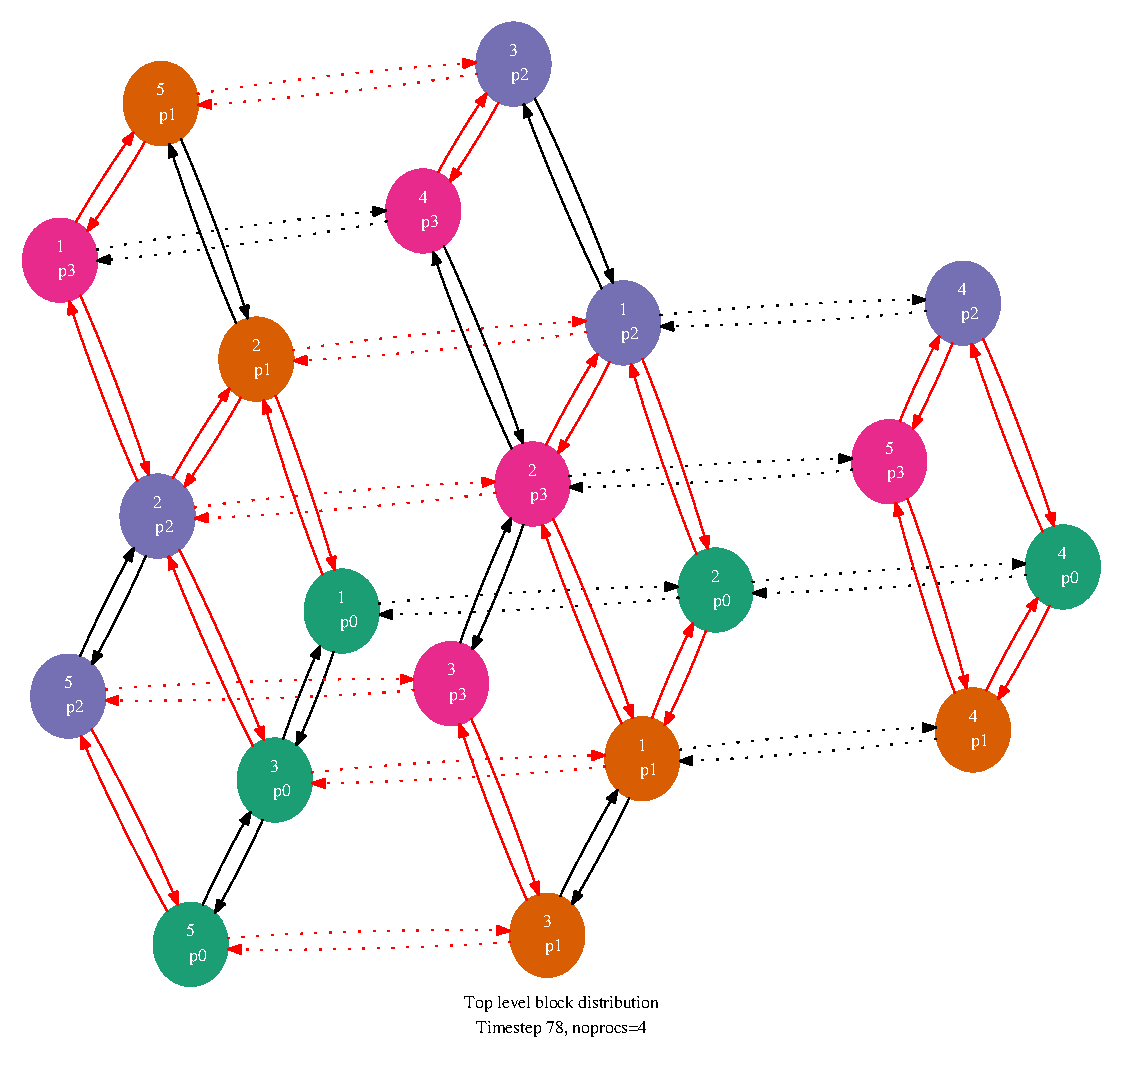
\includegraphics[width=8.0cm]{digraph.eps}
	\caption{Example figure produced using \texttt{blockGrapher} and \texttt{neato} of coarse grid blocks on a grown domain}
	\label{FIG_digraph}
\end{figure}

%%%%%%%%%%%%%%%%%%%%%%%%%%%%%%%%%%%%%%%%%%%%%%%%%%%%%%%%%%%%%%%%%%%%%%%%%%%%%%%%%%%%%%%%%%%%%%%%%%%%%%%%%%%%%%%%%%%%%%%%%%%%%%%%%%%%%%%%%%%%%%%%%%%%%%%%%%%%%%%%%%%

\section{Documentation}
								\label{SEC_Documentation}

Within Campfire is a directory called \texttt{DOCS}.  This, in turn, has subdirectories for each of the applications in addition to the source to this document 
itself.  
Building these documents is done using the command
\begin{codebox}
	\prompt{make DOCS}
\end{codebox}
and as new documents are added appropriate changes will be needed on the \texttt{Makefile}s encountered along the way.

As the models developed grow it is useful to store additional information, not easily captured n the code, such as derivations and justifications, in this 
central archive.  Indicating the location of these documents from comments in the code should be encouraged.



%%%%%%%%%%%%%%%%%%%%%%%%%%%%%%%%%%%%%%%%%%%%%%%%%%%%%%%%%%%%%%%%%%%%%%%%%%%%%%%%%%%%%%%%%%%%%%%%%%%%%%%%%%%%%%%%%%%%%%%%%%%%%%%%%%%%%%%%%%%%%%%%%%%%%%%%%%%%%%%%%%%

\section{API}
								\label{SEC_API}

The following functions are all called from within Campfire and need to be provided in the user code.  Many can just be stubs if not 
needed.  Obviously a domain needs initialisation and the user needs to provide an appropriate smoother and residual calculation routines (which 
will be very similar).

Initialisation:

\begin{itemize}
\item{\texttt{app\_parameter\_set}
 ( )}

\item{\texttt{app\_domain\_setup}
 (\texttt{pid}, \texttt{noprocs})}

\item{\texttt{app\_initial\_soln\_blk}
 (\texttt{lb})}

\item{\texttt{app\_initial\_soln\_end}
 ()}
\end{itemize}

Multigrid smoother and defect calculation:

\begin{itemize}
\item{\texttt{app\_mg\_smooth}
 (\texttt{pid}, \texttt{level})}

\item{\texttt{app\_mg\_get\_defect\_var}
 (\texttt{lb}, \texttt{max\_defect}, \texttt{rms}, \texttt{npts})}
\end{itemize}

Alternative local refinement routine:

\begin{itemize}
\item{\texttt{app\_test\_refinement}}
 ( )
\end{itemize}


Input/output:

\begin{itemize}
\item{\texttt{app\_read\_checkpoint}
 (\texttt{pid}, \texttt{noprocs})}

\item{\texttt{app\_pretimeloop\_output}
 (\texttt{pid}, \texttt{noprocs})}

\item{\texttt{app\_close\_files}
 (\texttt{pid}, \texttt{noprocs})}

\item{\texttt{app\_output\_perstep}
 (\texttt{pid}, \texttt{noprocs}, \texttt{stepno})}

\item{\texttt{app\_output\_occasional}
 (\texttt{pid}, \texttt{noprocs}, \texttt{stepno})}
\end{itemize}

There are also many variables stored in \texttt{MG-SRC/amr\_modules.f90} that are used across the software without being passed as arguments.
Brief descriptions of ones that may be set are given in the following table.

\begin{center}
	\begin{longtable}{|lc|p{0.6\textwidth}|}
		\hline
		\multicolumn{3}{|l|}{\texttt{multigrid\_parameters}}\\
		\hline
		\texttt{weight }& & Weight factor used in pointwise Jacobian Newton updates\\
		
		\texttt{smooth\_count\_max }& & How many pre/post smooth\\
		\texttt{solve\_count\_max	}& & How many smooths constitute a full solve\\
		\texttt{mg\_min\_lvl }& & Lowest (coarsest) refinement level which V-cycles go to\\
		\texttt{max\_v\_cycle\_count}& & Maximum number of V-cycles per timestep\\
  		\texttt{defect\_tol\_min  }& &Defect test for convergence of timestep \\
  		\texttt{defect\_too\_big }& &Final defect test for failing timestep\\
  		\texttt{defect\_tol\_max  }& &Intermediate defect test for failing timestep\\
  		\texttt{low\_vcycle\_count             }& &V-cycle count if has converged too easily\\
  		\texttt{high\_vcycle\_count            }& &V-cycle count if has converged too slowly\\

		\texttt{nunkvbles }& &   How many variables per variable\\
		\texttt{mg\_update\_total }& &Positive means will always fail test if not set\\
		\hline
		\multicolumn{3}{|l|}{\texttt{time\_dep\_parameters}}\\
		\hline
		\texttt{dt	}& & Default timestep size\\
		\texttt{max\_dt}& &  Max possible value of dt\\
		\texttt{min\_dt}& &  Min possible value of dt\\
		\texttt{simulation\_time }& &End time of simulation\\
		\texttt{max\_time\_iter}& &Maximum number of time-steps to take\\
		\texttt{shampine\_test}& &Use Shampine convergence test on each timestep (1=yes, 0=no)\\
		\texttt{shampine\_tol }& &Tolerance for Shampine convergence test\\

  		\texttt{stepsize\_increase\_frequency   }& & Every how often may timestep increases be imposed\\
		\texttt{tstep\_decrease\_factor}		&& Factor by which timestep is decreased\\
		\texttt{tstep\_increase\_factor}		&& Factor by which timestep is increased\\
  		\texttt{lee\_tol\_failing }& &Local error estimation tolerance for failing a timestep\\
  		\texttt{lee\_tol\_halving }& &Local error estimation tolerance for halving the stepsize\\
  		\texttt{lee\_tol\_decrease  }& & Local error estimation tolerance for decreasing the stepsize\\
  		\texttt{lee\_tol\_increase  }& & Local error estimation tolerance for doubling the stepsize\\
		\hline
		\multicolumn{3}{|l|}{\texttt{refinement\_parameters}}\\
		\hline
  		\texttt{allsolid\_test }& &   Are we doing the phase field case trying derefinement whenever all block values are 1 (1=yes, 0=no)\\
  		\texttt{ctore             }& & Error limit which controls refinement\\
  		\texttt{ctode            }& & Error limit which controls derefinement\\
		\hline
		\multicolumn{3}{|l|}{\texttt{checkpoint\_parameters}}\\
		\hline
  		\texttt{chk\_checkf }& & Style of checkpoint file `\texttt{default}' or '\texttt{HDF5}'\\
		\hline
                \multicolumn{3}{|l|}{\texttt{generic\_parameters}}\\
		\hline
		\texttt{local\_adaptation}& &  Will the amr\_test\_refinement and amr\_refine\_derefine calls be made?\\
		\texttt{numglobalref}& &  How many global refinements are needed initially?\\
		\texttt{grow }& & Will the domain be allowed to grow as needed? (1=yes, 0=no)\\
		\texttt{verbose}& &  Text output verbosity\\
		\texttt{output\_rate}& &  How often are the checkpoints, etc, produced in app\_output\_occasional\\
		\texttt{multigrid\_on}& & Is the multigrid solver to be used? (1=yes, 0=no, $>$1 means turn off after that many timesteps)\\
		\hline
	\end{longtable}
\end{center}

%%%%%%%%%%%%%%%%%%%%%%%%%%%%%%%%%%%%%%%%%%%%%%%%%%%%%%%%%%%%%%%%%%%%%%%%%%%%%%%%%%%%%%%%%%%%%%%%%%%%%%%%%%%%%%%%%%%%%%%%%%%%%%%%%%%%%%%%%%%%%%%%%%%%%%%%%%%%%%%%%%%

\section{Known Bugs and To Do list}
								\label{SEC_Bugs}

A full list of features and bugs is currerntly maintained in the ticketing system at \texttt{http://trac.leeds.ac.uk/EER-Campfire}.

\begin{itemize}
	\item{If mesh growing code is used then in parallel it seems to struggle finding coarsest neighbour initially if only a single block is used on the 
		coarsest level.  Clearly a single block with more than one level of refinement would need to grow anyway, so this may be a non-issue.}
	\item{Calls to \texttt{pf\_prolong} and \texttt{pf\_restrict} do not work correctly, so stick with  \texttt{amr\_prolong} and \texttt{amr\_restrict} for now.}
\end{itemize}


%%%%%%%%%%%%%%%%%%%%%%%%%%%%%%%%%%%%%%%%%%%%%%%%%%%%%%%%%%%%%%%%%%%%%%%%%%%%%%%%%%%%%%%%%%%%%%%%%%%%%%%%%%%%%%%%%%%%%%%%%%%%%%%%%%%%%%%%%%%%%%%%%%%%%%%%%%%%%%%%%%%
%%%%% References need making style consistent

\bibliographystyle{chris}
\begin{thebibliography}{10}
\bibitem{paramesh1}{ Peter MacNeice, Kevin M. Olson, Clark Mobarry, Rosalinda deFainchtein and Charles Packer, "PARAMESH : A parallel adaptive mesh refinement 
community toolkit.", Computer Physics Communications, vol. 126, p.330-354, (2000).}
\bibitem{paramesh2}{ Kevin Olson and Peter MacNeice, 2005, "An Over of the PARAMESH AMR Software and Some of Its Applications",in Adaptive Mesh Refinement-Theory 
and Applications, Proceedings of the Chicago Workshop on Adaptive Mesh Refinement Methods, Series: Lecture Notes in Computational Science and Engineering, vol. 41, 
eds. T. Plewa, T. Linde, and G. Weirs (Berlin: Springer).}
\bibitem{paramesh3}{ Kevin Olson, 2006, "PARAMESH: A Parallel Adaptive Grid Tool", in Parallel Computational Fluid Dynamics 2005: Theory and Applications: 
Proceedings of the Parallel CFD Conference, College Park, MD, U.S.A., eds. A. Deane, A. Ecer, G. Brenner, D. Emerson, J. McDonough, J. Periaux, N. Satofuka, and D. 
Tromeur-Dervout (Elsevier).}
\bibitem{parameshCode}{PARAMESH source code : \texttt{http://sourceforge.net/projects/paramesh/}}
\bibitem{janref1}{Mullis A M, Rosam, J and Jimack, P K, Solute Trapping and the effects of Anti-Trapping Currents on Phase-Field Models of Coupled Thermo-Solutal 
Solidification J. Cryst. Growth, vol.312, pp.1891--1897, 2010.}
\bibitem{janref2}{Rosam, J, Jimack, P K and Mullis, A M, Quantitative Phase-Field Modelling of Solidification at High Lewis Number . Physical Review E, vol.79, 
article 030601(R), 2009.}
\bibitem{janref3}{Rosam, J, Jimack, P K and Mullis, A M, An Adaptive, Fully Implicit, Multigrid Phase-Field Model for the Quantitative Simulation of Non-isothermal 
Binary Alloy Solidification. Acta Materialia, vol.56, pp.4559-4569, 2008. }
\bibitem{jancode}{PhAIM-2d : \texttt{http://www.digital.leeds.ac.uk/software}}
\bibitem{jamesref1}{Green, J, Jimack, P K, Mullis A M and Rosam, J, An Adaptive, Multilevel Scheme for the Implicit Solution of Three-Dimensional Phase-Field 
Equations Numerical Methods for PDEs, vol.27, pp.106--120, 2011. }
\bibitem{jamesref2}{Green, J R, Jimack, P K, Mullis, A M and Rosam, J, Towards a Three-Dimensional Parallel, Adaptive, Multilevel Solver for the Solution of 
Nonlinear, Time-Dependent, Phase-Change Problems. In Parallel, Distributed and Grid Computing for Engineering, eds. B.H.V. Topping and P. Ivanyi (Saxe-Coburg 
Publications, UK), pp.251--274, 2009.}
\end{thebibliography}
% ------------------------------------------------------------------------------ % End document 
%------------------------------------------------------------------------------ 
\end{document}
